% !TeX root = ../thuthesis-example.tex


%\chapter{论文主要部分的写法}
\chapter{Introduction}

\section{Background}
Representation learning \cite{bengio2013representation}, especially deep representation learning (or deep learning, DL), has become one of the most popular techniques since \citet{krizhevsky2012imagenet} developed a powerful deep neural network (DNN) that can significantly outperform shallow methods on ImageNet \cite{deng2009imagenet}. After that, DNN based methods have thrived in various machine learning domains, including computer vision \cite{simonyan2014very}, natural language processing \cite{kim-2014-convolutional}, recommendation \cite{cheng2016wide}, reinforcement learning \cite{silver2016mastering}, and so on. These works make a substantial progress in building better artifical intelligence (AI) applications by DNN. However, it remains elusive why DNN gains so much improvement with adding more layers of representations. This question encourages us to think of opening the black box of DNN.

In statistical learning theory \cite{vapnik2013nature} and probably approximately correct (PAC) learning theory \cite{valiant1984theory}, a too complex model suffers from \emph{over-fitting} problem thus failing in out-of-sample test. Recent work challenged them when the so-called benign over-fitting is observed in practice. That is, a hierarchical representation learning model with the number of parameters much more than the samples, i.e., \emph{over-parametrized}, still generalizes well on numerous tasks. This phenomenon ignites a surge of research under the theme of rethinking the generalization of representation learning \cite{zhang2016understanding}. One pitfall of the traditional learning theory is the lacking consideration of the input data distribution. 

Information theory \cite{cover1999elements} is a promising candidate for unveiling the black box in representation learning. A landmark in this line of research is using information bottleneck (IB) to model the learning process of DNN \cite{tishby2000information, tishby2015deep}. They utilized mutual information between the layers and the input and output variables to quantify DNN. It sheds light on characterizing generalization of representation learning by taking data distribution into account. After that, experiments showed that stochastic gradient descent (SGD) is capable of improving the generalization by compressing the redundant information contained in representations through the lens of IB \cite{shwartz2017opening}.

In information theory, IB was originally proposed as a means of finding minimal sufficient statistics. The minimality term in IB originates from the principle of minimum description length. In the sense of representation learning, IB describes a trade-off between the representation minimality and sufficiency.  The minimality term naturally works for a regularization term that urges the representation to generalize better. This property encourages a series of works in adopting IB for better representation learning. For example, by parameterizing the IB by variational inference, variational information bottleneck was proposed for yielding better generalization performance and robustness to adversarial attack of DNN in image classification \cite{alemi2016deep}. For this reason, it is quite surprising to see how IB could be used for more applications beyond the simple image classification task. In fact, we shall see that we can utilize IB for debasing recommender system models with a novel VI based approach. 

Moreover, in this paper, we explore a new perspective of information bottleneck. We look into a novel information-theoretic generalization measure that is built upon the mutual information between the learned weight and the selected finite-sample dataset. With this measure, we propose a new information bottleneck, namely PAC-Bayes information bottleneck (PIB), and give an MCMC based solution for approximate inference of the optimal posterior.

\section{Representation learning}
The success of machine learning algorithms heavily relies on the representation of data. Prior to the deep learning era, manual feature engineering is a necessary step for preprocessing the raw data and then completing effective machine learning. Representation learning, on the other hand, advocates to automatic learning of informative data representations when building classifiers or other predictors. These representations are encouraged to be informative to the underlying explanatory factors from inputs. As a result, they are expected to be useful for downstream tasks or further fine-tuned under supervision. Since then, the core concern is that how to design good objective functions for learning data representations.

Deep learning (DL) has drawn a great revolution in AI research in past ten years. While the depth is a key factors of the sucess of DL, it should be noted DL is still a subset of the conception of representation learning, in other words, we would prefer to call deep learning as \emph{deep representation learning} for preciseness. For example, Word2Vec was proposed to reduce the number of parameters required by the the re-use of parameters  \cite{mikolov2013distributed}. Unlike the common deep learning setting, this distributed representation learning paradigm does not have multiple layers.

As the name indicates, one key characteristic of deep learning is its depth. Two high-level ideas are that the deep hierarchical architecture promotes the \emph{re-use} of features and improve the feature \emph{abstraction} at the tail near the final output \cite{bengio2013representation}. When the number of layers grows, the number of possible paths grows exponentially. This feature allows computational efficiency of DNN in the universal approximation of arbitrary functions. That is, using deeper models can reduce the number of units required to represent the desired function and can reduce the amount of generalization error \cite{goodfellow2016deep}. On the other hand, the hierarchy of features enables the composition of fundamental concepts towards abstract objects. Generally, more abstract features are more invariant to the local variation of inputs. The invariance thus allowing the excellent predictive power of learned representations. 

However, beyond this perceptual understanding of DL, there are still questions waiting for answers. For example, why stochastic gradient descent (SGD) can encourage both efficient and effective training of DNNs? To what extent different batch size influences the generalization of the learned DNNs? On account of them, We follow the idea of casting our eyes on another toolkit, e.g., information theory, to help us understand and design representation learning algorithms throughout this paper.


\section{Information bottleneck}
In the learning problem, information theory provides a quantitative notion of ``relevant" information, defined by the mutual information $I(X;Y)$ as
\begin{equation}
    I(X;Y) \triangleq \int \int p(x,y) \log \frac{p(x,y)}{p(x)p(y)} dx dy.
\end{equation}
With the input feature $X$ and the target signal $Y$, our object of interest is to extract the information contained in $X$ that is relevant to the target $Y$ by an intermediate representation $T$, i.e., $I(X;Y)=I(T;Y)$.  It could be seen that a trivial way to obtain all the relevant information is just making $T$ an identical mapping. Under the context of information theory, this is often formulated as a ``rate distortion" problem that characterizes the tradeoff between the size of representation, and the average distortion of the reconstructed signal \cite{cover1999elements}. Apart from the target, we design another target to restrict the irrelevant information by minimizing the mutual information $I(X;T)$. We thus build an optimization problem
\begin{equation} \label{eq:mss}
    \min_T I(T;X), \ \text{s.t.} \ I(T;Y)=I(X;Y).
\end{equation}
By solving this problem, we obtain the \emph{simplest} representation of $X$ while still maintain all relevant information of $Y$. In statistical term, the obtained $T$ is thus called \emph{minimal sufficient statistics} (MSS).

\begin{figure}[t]
  \centering
  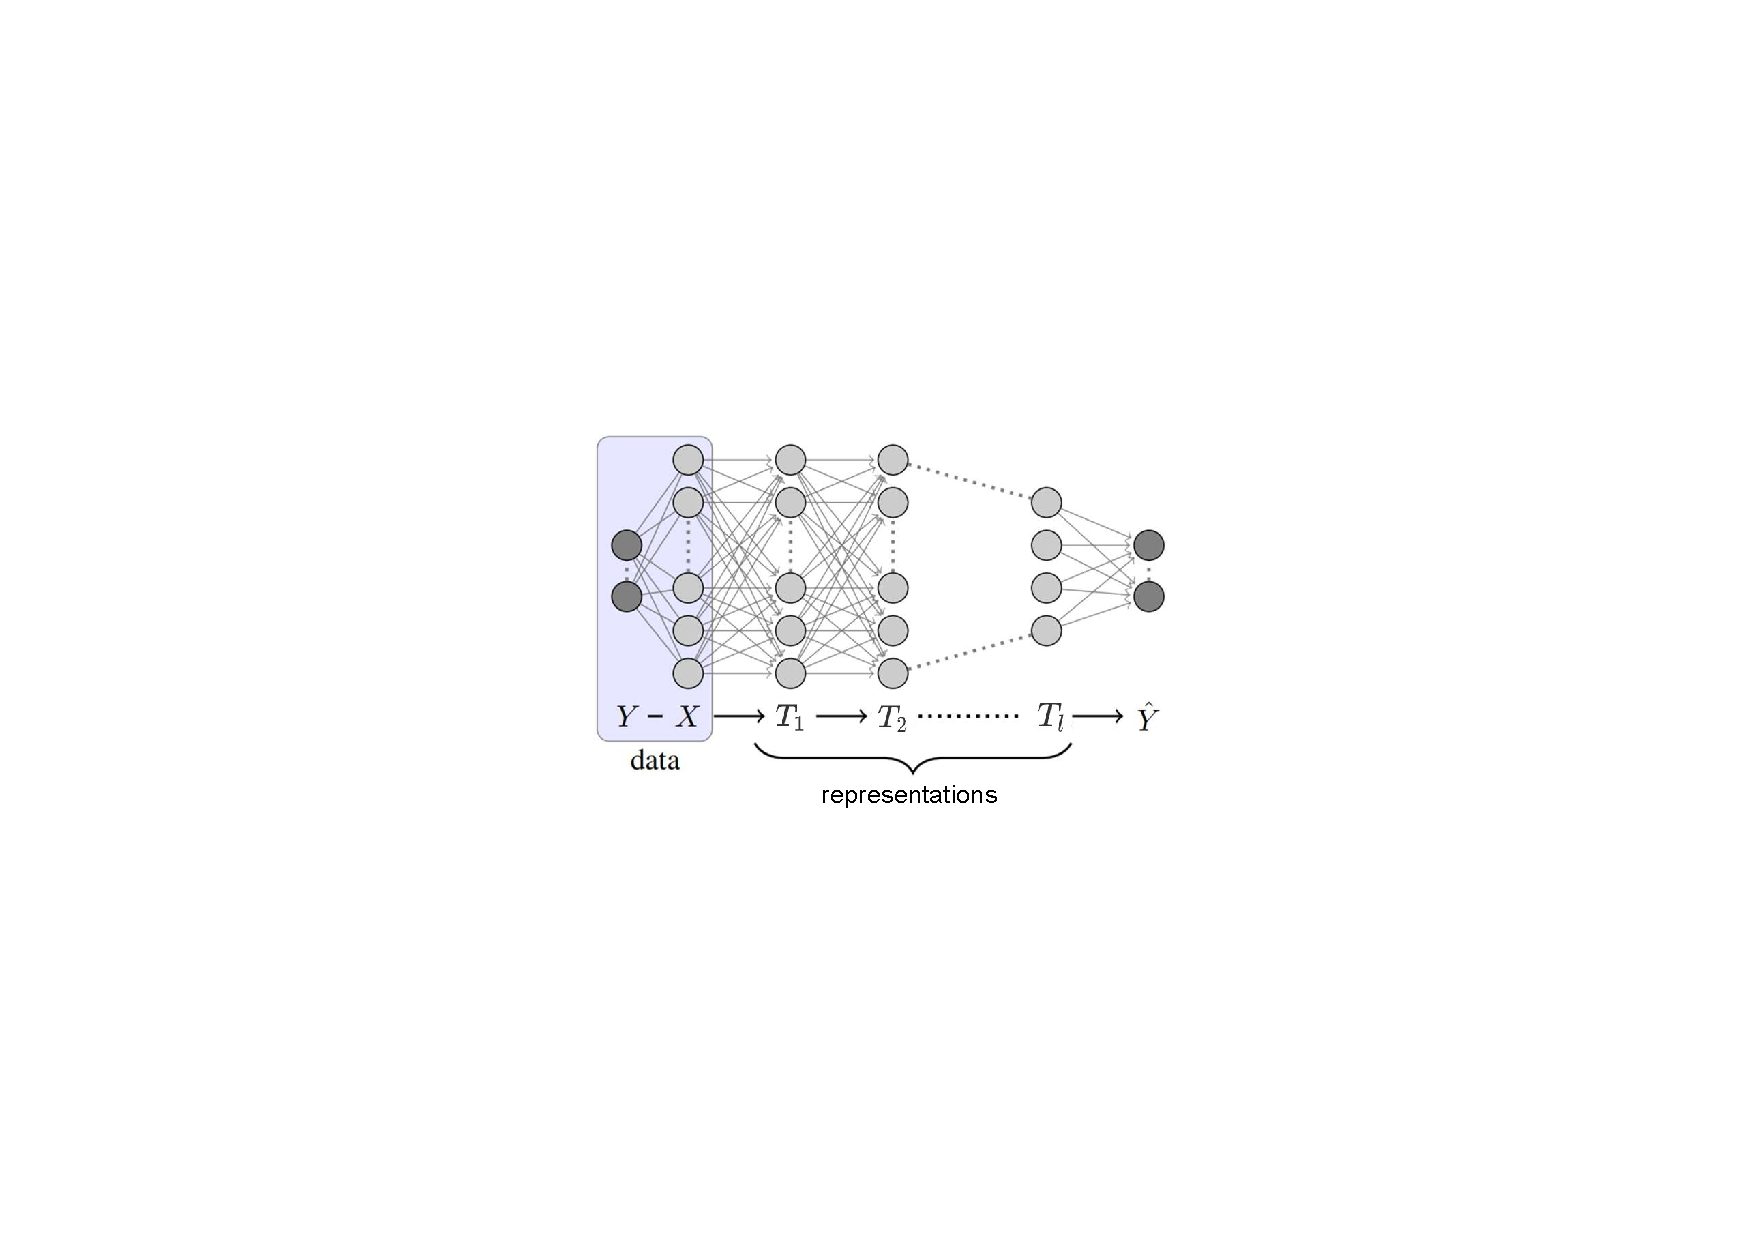
\includegraphics[width=0.6\linewidth]{fig1.pdf}
  \caption{A hierarchy of representations in DNN is formulated as a Markov chain, reproduced from \inlinecite{tishby2015deep}.}
  \label{fig:hierarchy_dnn}
\end{figure}

In this setting, we view the information processing of $X$ as a Markov chain that
\begin{equation}
 Y \to X \to T \to \hat{Y}.
\end{equation}
For a general distribution $p(X,Y)$, however, the MSS might even not exist and the problem in Eq. \eqref{eq:mss} becomes insolvable. On consideration of this challenge, \citet{tishby2000information} proposed a Lagrangian relaxation of the original problem, to build a bottleneck as
\begin{equation}
 \mathcal{L}_{\text{IB}} =  I(X;T) - \beta I(T;Y),
\end{equation}
where $\beta$ is Lagrangian multiplier operates a hyperparameter that controls the tradeoff of regularization and sufficiency.

When there are multiple layers of representations, this Markov chain is also extended such that $X \to T_1 \to T_2 \dots T_l$ as $l$ is the total number of layers, shown by Fig. \ref{fig:hierarchy_dnn}. According to the data processing inequality (DPI), we know that $I(T_1;X) \geq I(T_2;X) \geq \dots I(T_l;X)$.



\emph{in this work we focus on design principled information bottleneck method for representation learning. This method can also be applied for DNN with minimal adaptions in case of computational efficiency.}


\section{Literature review}

\emph{Explaining deep learning through the lens of information}

\section{Thesis structure}

